\section*{Assignment 07: Inequality and Responsibility}
\addcontentsline{toc}{section}{Assignment 07: Inequality and Responsibility}

First I map who falls through the cracks. Resource-light NGOs lack cash and staff to babysit another dashboard and fear hidden fees or data obligations \citep{Srnicek2017}. Humanities and design faculties also risk being sidelined because their success metrics differ from the business-school crowd, echoing \citet{Choudary2016}'s reminder that governance must match each segment’s value logic and reinforcing the inequality lens from Lecture~8 \citep{Lecture08}.

The core initiatives follow three tracks:
\begin{itemize}
  \item \textbf{Resource-light NGOs}: Lean onboarding kit with templated briefs, a co-piloted first sprint, and auto-generated reports so they launch projects without extra staff \citep{Gunasilan2024}.
  \item \textbf{Humanities and design faculties}: ``Faculty sandboxes'' with custom metrics, analogue upload options, and shared moderation guidelines \citep{Reillier2017}.
  \item \textbf{Cross-campus community}: Fairness clause, inclusion council, and quarterly impact audit to make data use transparent \citep{ShapiroVarian1999,Rennella2023}.
\end{itemize}

To make life easier for NGOs we roll out the lean onboarding kit: a ready-made data sheet, templated briefs, and a buddy system that pairs them with students during the first weeks. The VirtuAI case showed how crucial that social onboarding layer is when resources are thin \citep{Gunasilan2024}, and automated reports plus budget caps let organisations skip building measurement tools from scratch.

For faculties the move is to let them shape their own micro-communities. ``Faculty sandboxes'' let humanities define alternative engagement metrics while economists keep classic growth curves, mirroring \citet{Reillier2017}'s advice on modular governance. Analogue experiments can be documented through simple uploads instead of mandatory livestreams.

Policy-wise I sketch three rules. First, a fairness clause tracks resource spend per organisation and offers fee waivers when volunteer hours pass a threshold, dovetailing with \citet{ShapiroVarian1999}. Second, an inclusion policy grants every faculty a seat on a data-and-ethics council to avoid governance bias, echoing \citet{Zuboff2019} and our Lecture~11 debate \citep{Lecture11}. Third, a recurring impact audit inspired by DineTogether reviews whether features inadvertently favour resource-rich actors each quarter \citep{Rennella2023}. All three policies sit inside the Terms of Use so commitments are binding rather than optional.

As an overarching design principle I stick with ``progressive engagement'': the more resources an actor has, the more advanced tools we unlock while the baseline stays simple and free. It operationalises balanced network effects so NGOs with minimal budgets and faculties with divergent success criteria can join without feeling overwhelmed, while ambitious partners still see a path to deeper collaboration.

Figure~\ref{fig:chat-system} captures the messaging system behind this fairness work: the interface handles micro-coaching, inclusion triage, and governance updates in plain language. Students can flag ``access support needed,'' NGOs can request translation help, and templated replies reference our fairness clause so tone stays consistent when moderators rotate.

\begin{figure}[H]
  \centering
  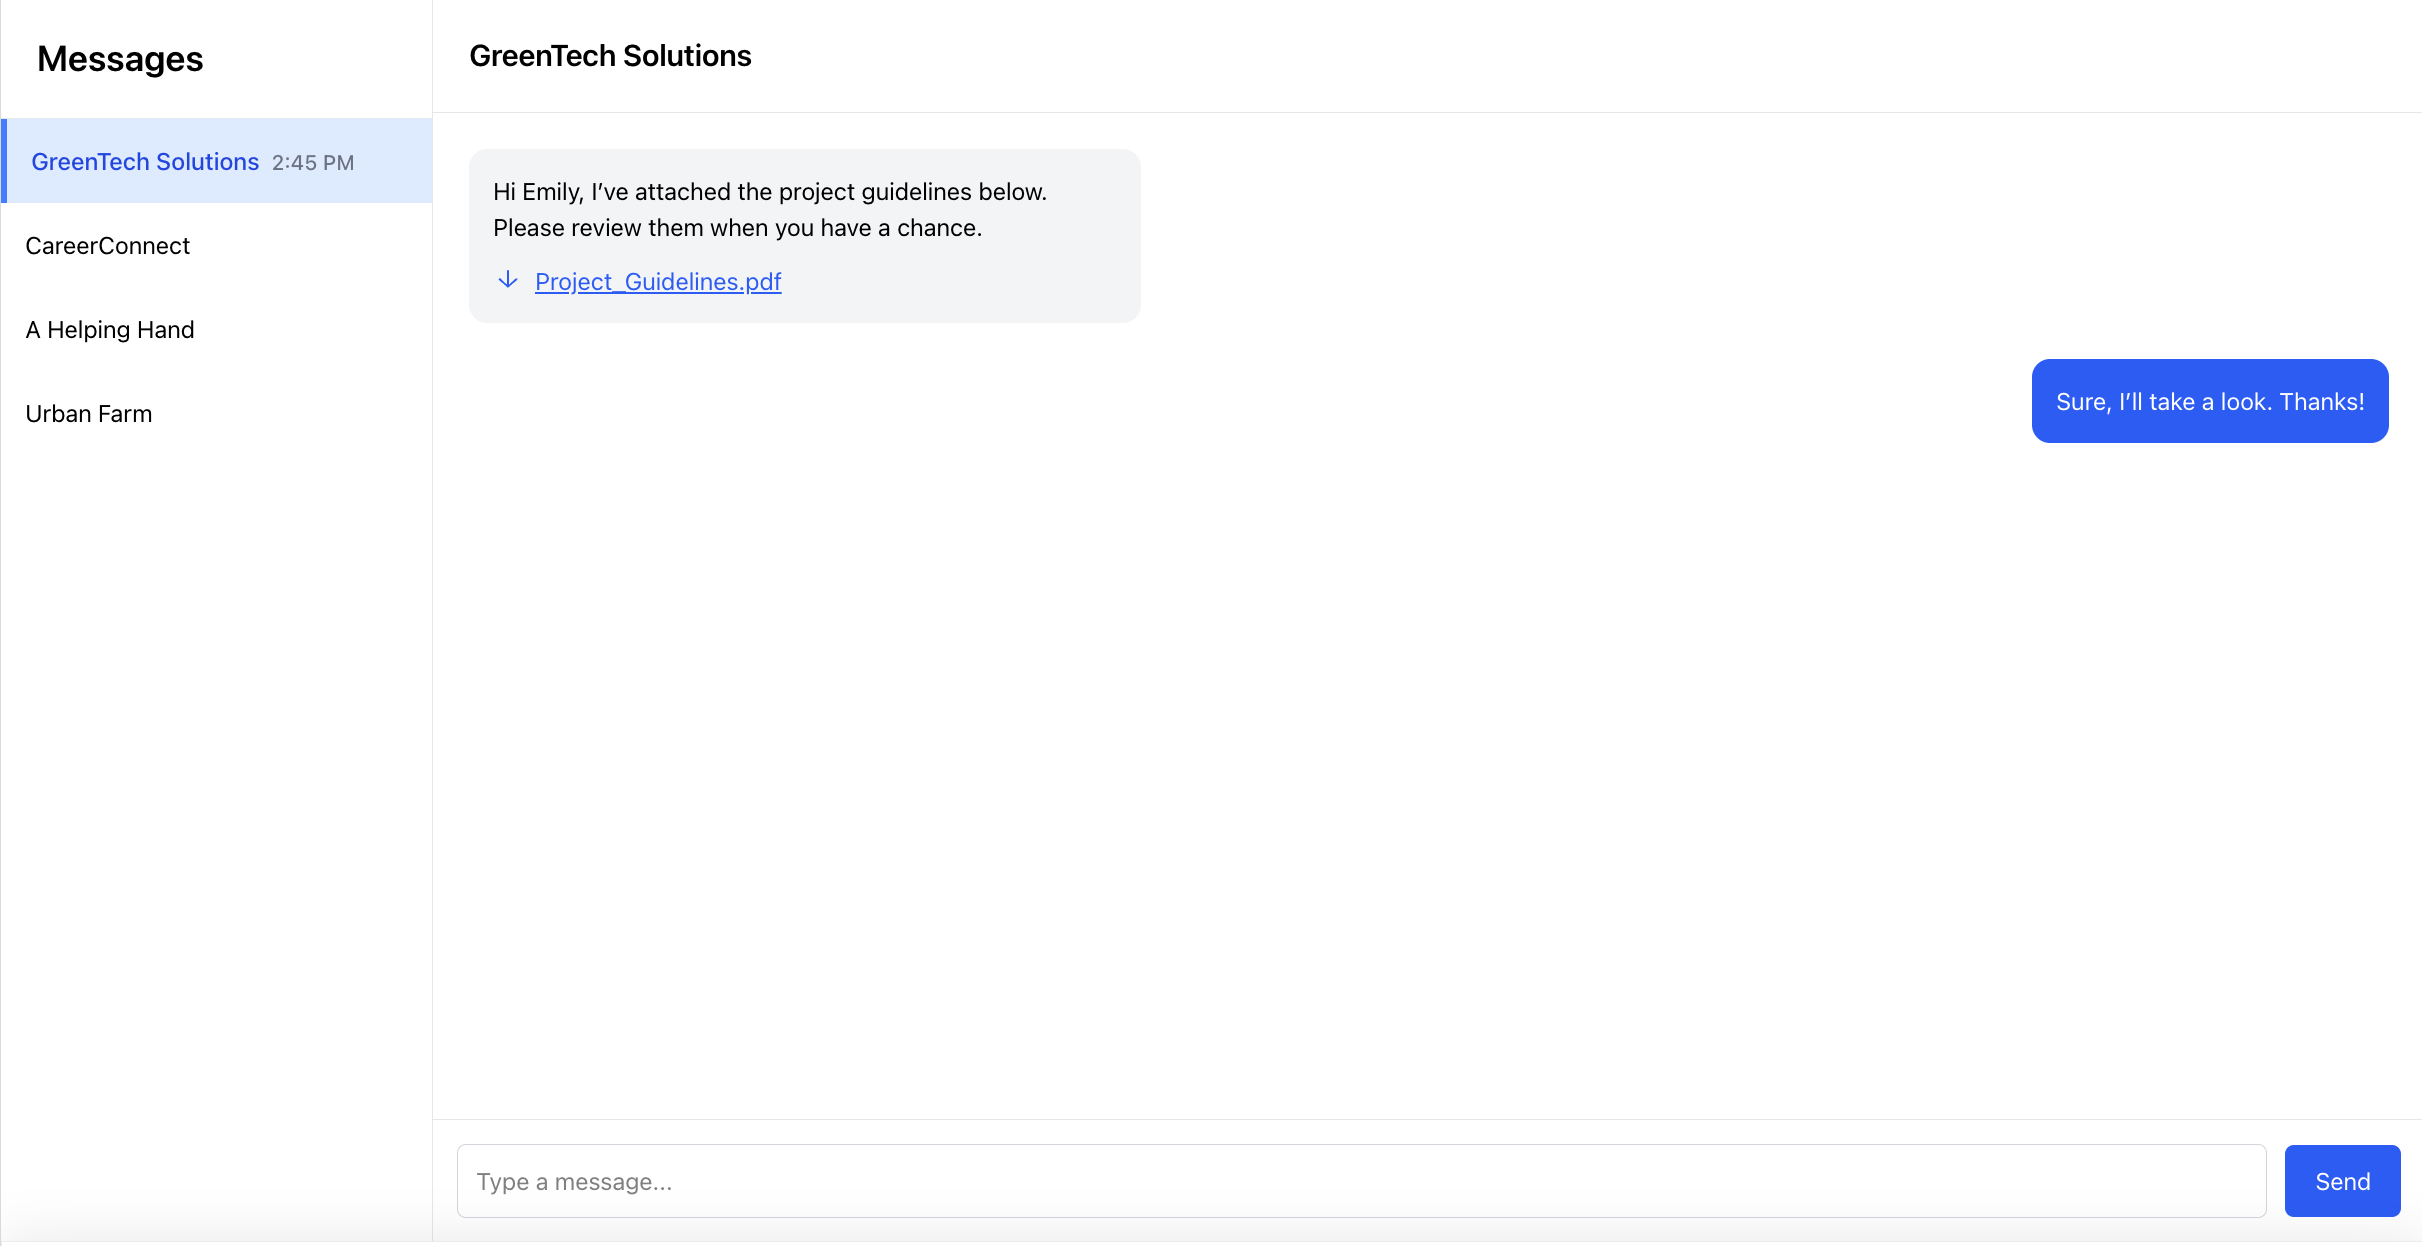
\includegraphics[width=0.85\linewidth]{Messengersystem.png}
  \caption{Messaging workspace coordinating inclusion support.}
  \label{fig:chat-system}
\end{figure}

I also introduced a ``mutual aid'' feature where resource-rich partners volunteer surplus capacity (design time, translation, data access) to NGOs with bandwidth gaps. The chat system coordinates offers, logs credits, and routes recognition so inequality does not harden as we scale \citep{Lecture09}.
